\section{Garbage Collection}
\textbf{Typ-Deskriptor Zweck}
\begin{itemize}
    \item Ancestor Table für Typ-Test \& Cast
    \item Virtual Method Table für Dynamic Dispatch
    \item Interpreter Metadata bei Field- / Array Typen
    \item \textbf{Neu:} Pointer Offsets für Garbage Collection
\end{itemize}

\subsection{Explizite Freigabe}
\begin{itemize}
    \item Delete Statement zum Deallozieren eines Objektes
\end{itemize}
\subsubsection{Probleme}
\begin{itemize}
    \item Dangling Pointers: Referenz auf gelöschtes Objekt
    \item Memory Leaks: Verweiste Objekte, die nicht abräumbar sind
\end{itemize}

\subsubsection{Dangling Pointer}
\begin{itemize}
    \item Zeigt auf Lücke oder falsches Objekt im Heap
    \item Lese nicht berechtigten Speicher (Security Issue)
    \item Überschreibe fremden Speicher (Safety + Security Issue)
\end{itemize}

\subsubsection{Memory Leak}
\begin{itemize}
    \item Unbenötigtes Objekt, das nicht löschbar ist
    \item Es gibt keine benutzbaren Referenzen mehr darauf
\end{itemize}

\subsection{Garbage Collection}
\begin{itemize}
    \item Laufzeitsystem kümmert sich um die automatische Freigabe von Garbage
    \item Garbage = Objekte, die nicht mehr erreichbar sind und daher nicht mehr gebraucht werden
\end{itemize}
\textbf{Ziel:}
\begin{itemize}
    \item Memory Safety
    \item Keine Dangling Pointers
    \item Keine Memory Leaks
\end{itemize}

\subsubsection{Reference Counting}
\begin{itemize}
    \item RC pro Objekt
    \item Anzahl eingehender Referenzen
    \item Zyklische Objektstrukturen werden mit Reference Counting nie zu Garbage
\end{itemize}
\textbf{Vorteil}
\begin{itemize}
    \item Sofortige Deallokation
\end{itemize}
\textbf{Nachteile}
\begin{itemize}
    \item Falsch bei Zyklen
    \item Ineffizient
\end{itemize}
\textbf{\textcolor{red}{Untauglich}}

\subsubsection{Transitive Erreichbarkeit}
\begin{itemize}
    \item Objekte beibehalten, die das Programm noch zugreifen könnte
    \item Ausgehend von Ankerpunkten (Root Set)
\end{itemize}
\textbf{Root Set}
\begin{itemize}
    \item Referenzen in statischen Variablen
    \item Referenzen in Activation Frames auf Call Stack
    \item Referenzen in Register
\end{itemize}

\subsection{Mark \& Sweep Algorithmus}
\textbf{Mark Phase}
\begin{itemize}
    \item Markiere alle erreichbaren Objekte
\end{itemize}
\textbf{Sweep Phase}
\begin{itemize}
    \item Lösche alle nicht markierten Objekte
\end{itemize}
\subsubsection{Mark Phase}
\begin{lstlisting}
private void mark() {
    for(var root: getRootSet(stack)) {
        traverse(root);
    }
}

private void traverse(Pointer current) {
    if(current == null) {
        return;
    }
    long block = heap.getAddress(current) - Heap.BLOCK_HEADER_SIZE;
    if(!isMarked(block)) {
        setMark(block);
        for(var next: getPointers(current)) {
            traverse(next);
        }
    }
}
\end{lstlisting}

\subsubsection{Rekursive Traversierung}
\begin{itemize}
    \item GC braucht zusätzlich Speicher für Stack
    \item Problematisch, da Speicher bei GC meist sowiso knapp ist
    \item Es exisitieren Algorithmen zur Traversierung ohne Zusatzspeicher (Pointer Rotation Algo)
\end{itemize}

\subsubsection{Sweep Phase}
\begin{itemize}
    \item Linearer Scan über den gesamten Heap, alle Blöcke
\end{itemize}
\begin{lstlisting}
private void sweep() {
    var current = Heap.HEAP_START;
    while(current < Heap.HEAP_SIZE) {
        if(!isMarked(current) && !freeList.contains(current)) {
            free(current);
        }
        clearMark(current);
        current += heap.getBlockSize(current);
    }
}

private void free(long address) {
    freeList.add(address);
}
\end{lstlisting}

\subsection{Ausführungszeitpunkt}
\textbf{Delayed Garbage Collection}
\begin{itemize}
    \item Garbage wird nicht sofort erkannt und freigegeben
    \item GC läuft spätestens, wenn der Heap voll ist (Check beim Allozieren)
    \item Eventuell prophylaktisch früher
\end{itemize}

\subsection{Stop \& Go}
\begin{itemize}
    \item GC läuft sequentiell und exklusiv
    \item Mutator = Produktives Programm
    \item Mutator ist während GC unterbrochen
\end{itemize}
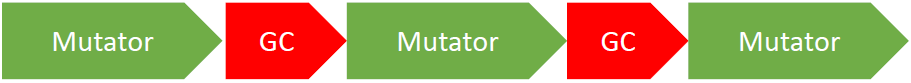
\includegraphics[width=0.6\linewidth]{stop_go.png}

\subsection{Root Set Erkennung}
\textbf{Pointer auf dem Call Stack}
\begin{itemize}
    \item Pointers in Parameter
    \item Pointers in lokalen Variablen
    \item Pointers auf Evaluation Stack
    \item this-Referenz
\end{itemize}

\subsection{Pointers im Objekt}
\begin{lstlisting}
private Iterable<Pointer> getPointers(Pointer current) {
    var list = new ArrayList<Pointer>();
    var descriptor = heap.getDescriptor(current);
    if(descriptor instanceof ClassDescriptor classDescriptor) {
        var fields = classDescriptor.getAllFields();
        for(var i = 0; i < fields.length; i++) {
            var type = fields[i].getType();
            if(isPointerType(type)) {
                var value = heap.readField(current, i);
                if(value != null) {
                    list.add((Pointer) value);
                }
            } 
        }
    } else if (descriptor instanceof ArrayDescriptor arrayDescriptor) {
        var length = heap.getArrayLength(current);
        for (int i = 0; i < length; i++) {
            var value = heap.readElement(current, i);
            var type = arrayDescriptor.getElementType();
            if (value != null && isPointerType(type)) {
                list.add((Pointer)value);
            }
        }
    }
    return list;
}

private boolean isPointerType(Object pointer) {
    return pointer instanceof ClassDescriptor || pointer instanceof ArrayDescriptor;
}
\end{lstlisting}

\subsection{Free List}
\begin{itemize}
    \item Freie Blöcke linear verketten
\end{itemize}
\subsubsection{Neue Heap Allozierung}
\begin{itemize}
    \item Traversiere Free List bis zu passendem Block
    \item Überschuss des Blockes wieder in free List einreihen
\end{itemize}
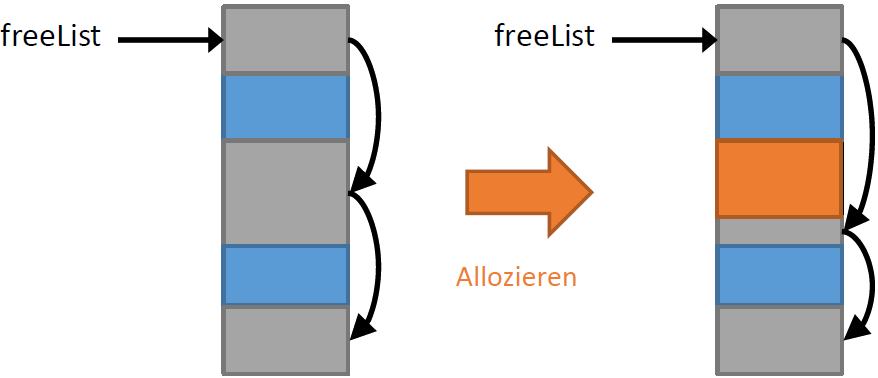
\includegraphics[width=0.6\linewidth]{free_list.png}
\subsubsection{Heap Block Layout}
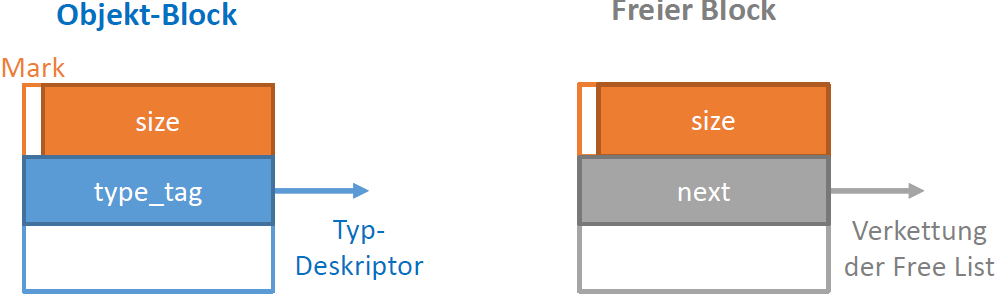
\includegraphics[width=0.6\linewidth]{heap_block_layout.png}
\subsubsection{Strategien}
\textbf{First Fit}
\begin{itemize}
    \item Keine Sortierung
    \item Suche erst passenden Block
\end{itemize}
\textbf{Best Fit}
\begin{itemize}
    \item Nach aufsteigender Grösse sortiert
    \item Unbrauchbar kleine Fragmente
\end{itemize}
\textbf{Worst Fit}
\begin{itemize}
    \item Nach absteigender Grösse sortiert
    \item Finde passenden Block sofort
\end{itemize}
\textbf{Segregated Free List}
\begin{itemize}
    \item Mehrere Free Lists mit verschiedenen Grössenklassen
    \item e.g. 64..128, 128..196, 196..259, ...
\end{itemize}
\textbf{Benachbarte freie Blöcke verschmelzen}
\begin{itemize}
    \item Am einfachsten in der Sweep Phase
\end{itemize}
\textbf{Buddy System}
\begin{itemize}
    \item Diskrete Blockgrössen nach Adresse geordnet
    \item Exponentielle Blockgrösse
    \item Sehr schnelles Verschmelzen \& Allozieren \& Freigabe
    \item Aber grosse interne Fragmentierung (unbrauchbare Reste)
\end{itemize}

\section{GC Vertiefung}
\textbf{Pointers in C++}
\begin{itemize}
    \item expliziter Zahlenwert
    \item Jedes Wort kann Pointer sein
    \item Keine GC Metadaten in C/C++
\end{itemize}

\subsection{Finalizer}
\begin{itemize}
    \item Methode, die vor Löschen des Objektes läuft (Abschlussarbeit wie z.B. Verbindung schliessen)
    \item Von GC initiiert, wenn Objekt Garbage geworden ist
\end{itemize}
\begin{lstlisting}
class Block {
    @Override 
    protected void finalize() {
        // ...
    }
}
\end{lstlisting}
\subsubsection{Separate Finalisierung}
\begin{itemize}
    \item Finalizer wird nicht in GC-Phase ausgeführt, sondern erst später
\end{itemize}
\textbf{Gründe}
\begin{itemize}
    \item Finalizer dauert evtl. beliebig lange (blockiert sonst GC)
    \item Finalizer kann neue Objekte allozieren (korrumpiert GC)
    \item Programmierfehler im Finalizer (evtl. Crash des GC)
    \item Finalizer kann Objekt wieder weiterleben lassen (Resurrection)
\end{itemize}

\subsubsection{Resurrection}
\begin{itemize}
    \item Finalizer kann bewirken, dass Objekt wieder lebendig wird und kein Garbage mehr ist
    \item Nicht nur das eigene Objekt, sondern auch indirekt andere Objekte können wiederauferstehen
\end{itemize}
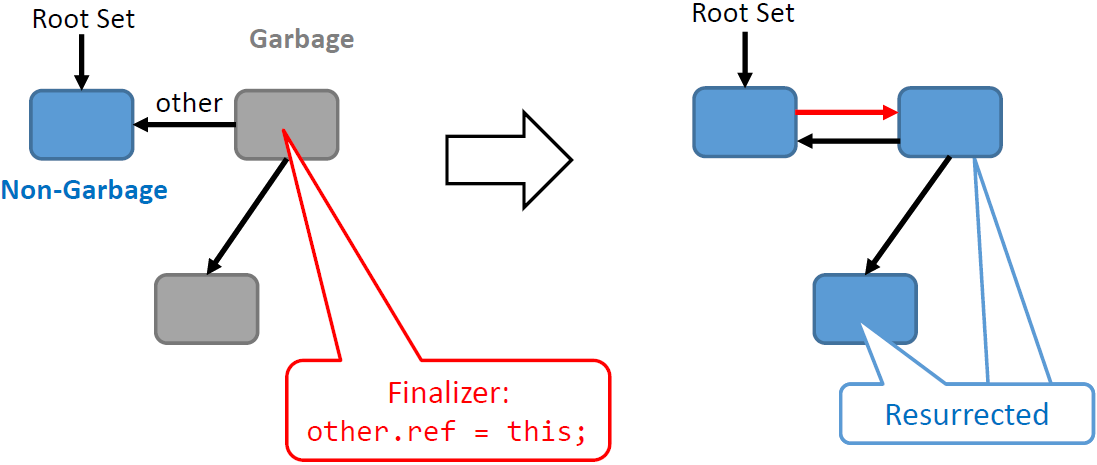
\includegraphics[width=0.6\linewidth]{resurrection.png}

\subsubsection{Internals}
\textbf{Finalizer Set}
\begin{itemize}
    \item Registrierte Finalizer
\end{itemize}
\textbf{Pending Queue}
\begin{itemize}
    \item Noch auszuführende Finalizer
    \item Garbage mit Finalizer werden in Pending Queue eingetragen
    \item Einfügen bewirkt Resurrection: Neue GC Phase nötig
\end{itemize}

\subsubsection{Konsequenzen}
\textbf{GC braucht 2 Mark Phasen}
\begin{itemize}
    \item Markiere und erkenne Garbage mit Finalizer
    \item Markiere von Pending Queue erneut, dann Sweep
\end{itemize}
\textbf{Objekt mit Finalizer braucht min 2 GC Durchläufe bis zur Freigabe}
\begin{itemize}
    \item Speicher kann evtl. nicht schnell genug frei werden
\end{itemize}

\subsubsection{Programmieraspekte}
\begin{itemize}
    \item Reihenfolge der Finalizer ist unbestimmt
    \item Laufen beliebig verzögert
    \item Sind nebenläufig zum Hauptprogramm
\end{itemize}

\subsection{Weak Reference}
\begin{itemize}
    \item Zählt nicht als Referenz für GC
    \item Für Objekt Caches
\end{itemize}
\textbf{Internals}
\begin{itemize}
    \item Indirektion via Weak Reference Table
    \item GC Mark ignoriert Table-Einträge
    \item GC Sweep nullt Einträge, falls Zielobjekte gelöscht
\end{itemize}

\subsection{Externe Fragmentierung}
\textbf{Viele kleine Lücken im Heap durch Allozieren \& Free}
\begin{itemize}
    \item Spätere grössere Allokation passt in keine Lücke
    \item Obschon Summe der freien Blöcken genügend wäre
\end{itemize}
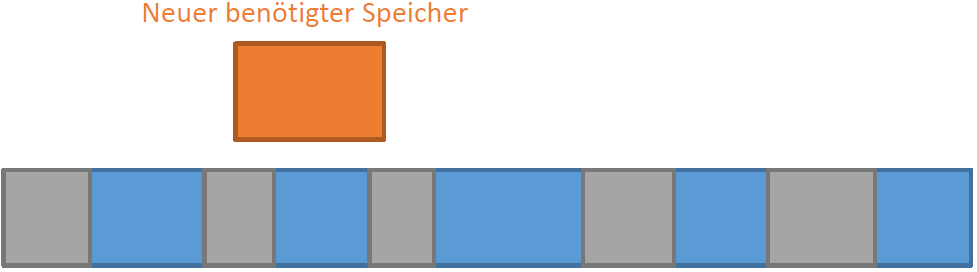
\includegraphics[width=0.6\linewidth]{externe_frag.png}

\subsection{Compacting GC}
\begin{itemize}
    \item Auch Mark \& Copy GC
    \item Allokation am Heap-Ende (supereffizient)
    \item GC schiebt Objekte wieder zusammen
    \item Bei Verschieben müssen Referenzen nachgetragen werden
    \item Konservative Methode daher unmöglich (C/C++ nicht möglich)
\end{itemize}
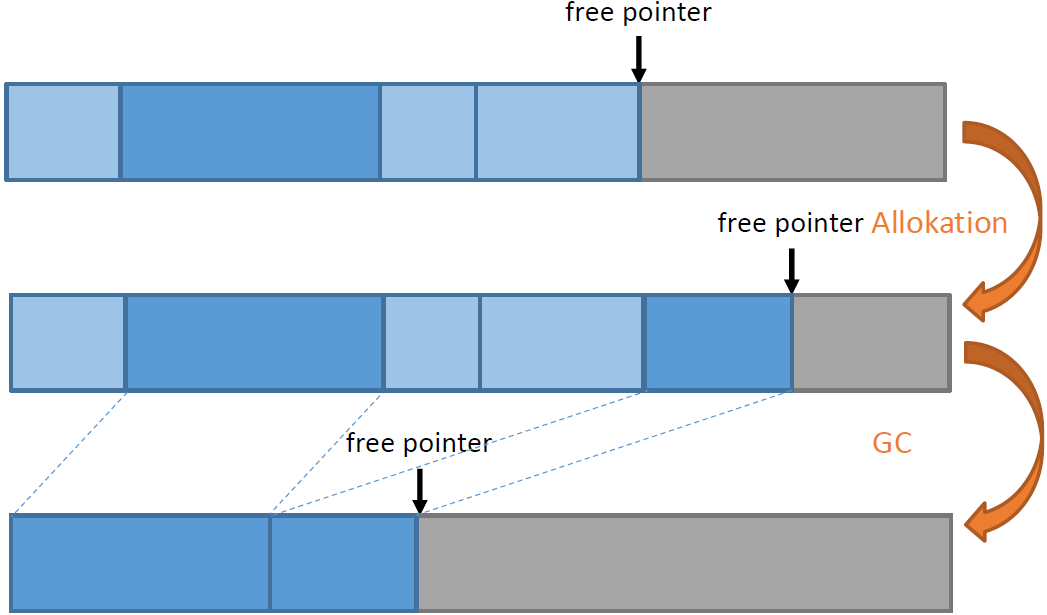
\includegraphics[width=0.5\linewidth]{compacting_gc.png}

\subsection{Inkrementeller GC}
\begin{itemize}
    \item GC soll quasi-parallel zum Mutator laufen
    \item Nur kleinste Unterbrüche (Inkrements)
    \item Kein Stop \& Go / Stop the World
\end{itemize}
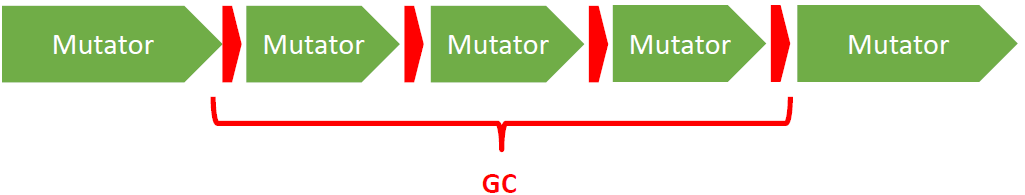
\includegraphics[width=0.6\linewidth]{inkr_gc.png}
\subsubsection{Generational GC}
\textbf{Zeitspiegelungsheuristik}
\begin{itemize}
    \item Junge Objekte: kurze Lebensdauer
    \item Alte Objekte: lange Lebensdauer
\end{itemize}
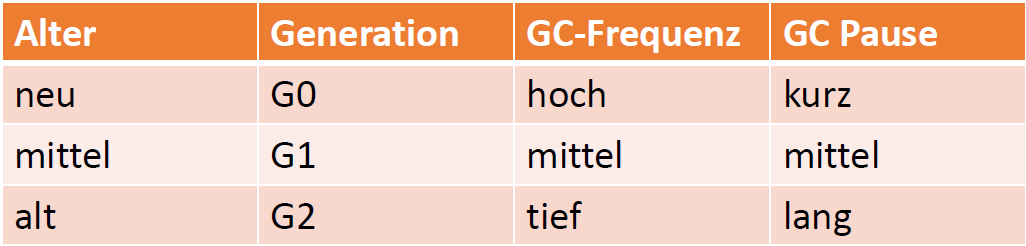
\includegraphics[width=0.5\linewidth]{generational_gc.png}\\
\textbf{Root Sets bei Generationen}
\begin{itemize}
    \item Referenzen von alten zu neuen Generationen: Zusätzlicher Root Set der neuen Gen
    \item Write Barriers: Schreiben von Referenzen in alte Generationen erkennen
    \item Bei GC der alten Generationen müssen auch neuere mit aufgeräumt werden
\end{itemize}

\subsubsection{Partitioned GC}
\begin{itemize}
    \item Heap in Partitionen zerlegen
    \item Ziel: kurze GC Pausen
    \item Nebenläufiges Markieren mit Snapshots: Relevante nebenläufige Updates erkennen
    \item GC fokussiert auf Partitionen mit viel Garbage
    \item Evakuiere lebende Objekte in neue Partitionen
\end{itemize}
\textbf{Problem}
\begin{itemize}
    \item Zyklischer Garbage zwischen Partitionen
    \item Braucht immer noch Full GC (Stop the World)
\end{itemize}
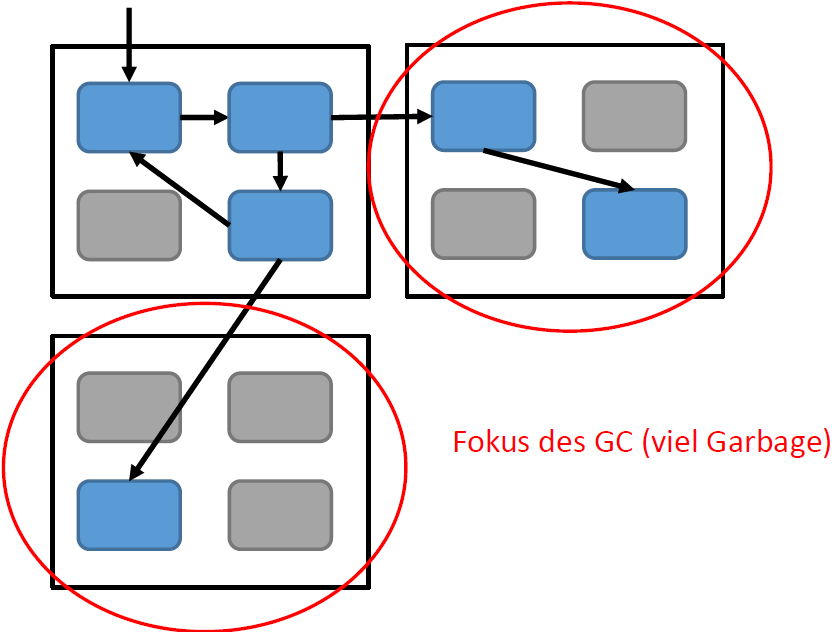
\includegraphics[width=0.3\linewidth]{partitioned_gc1.png} $\rightarrow$
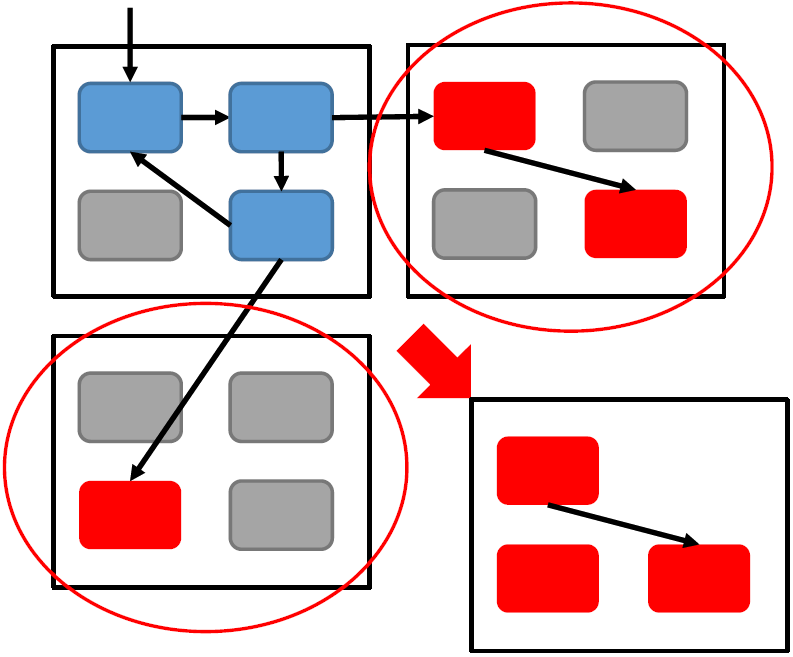
\includegraphics[width=0.3\linewidth]{partitioned_gc2.png} $\rightarrow$
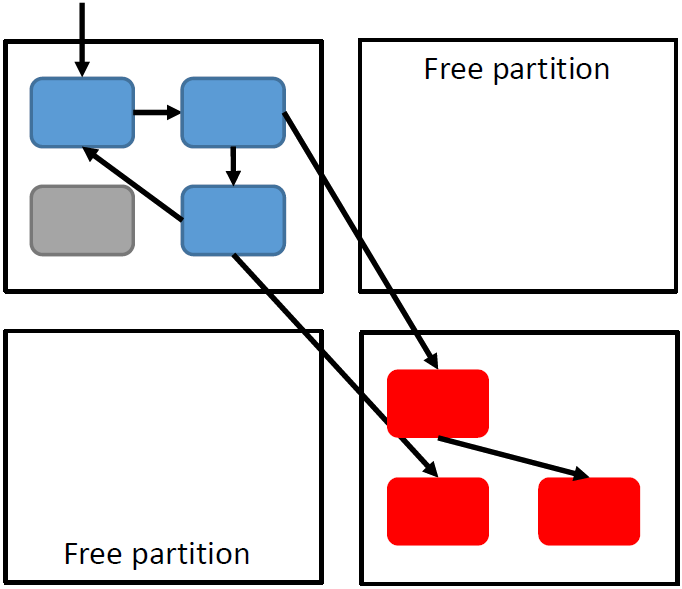
\includegraphics[width=0.3\linewidth]{partitioned_gc3.png}

\subsection{Wellenausbreitungsmodell}
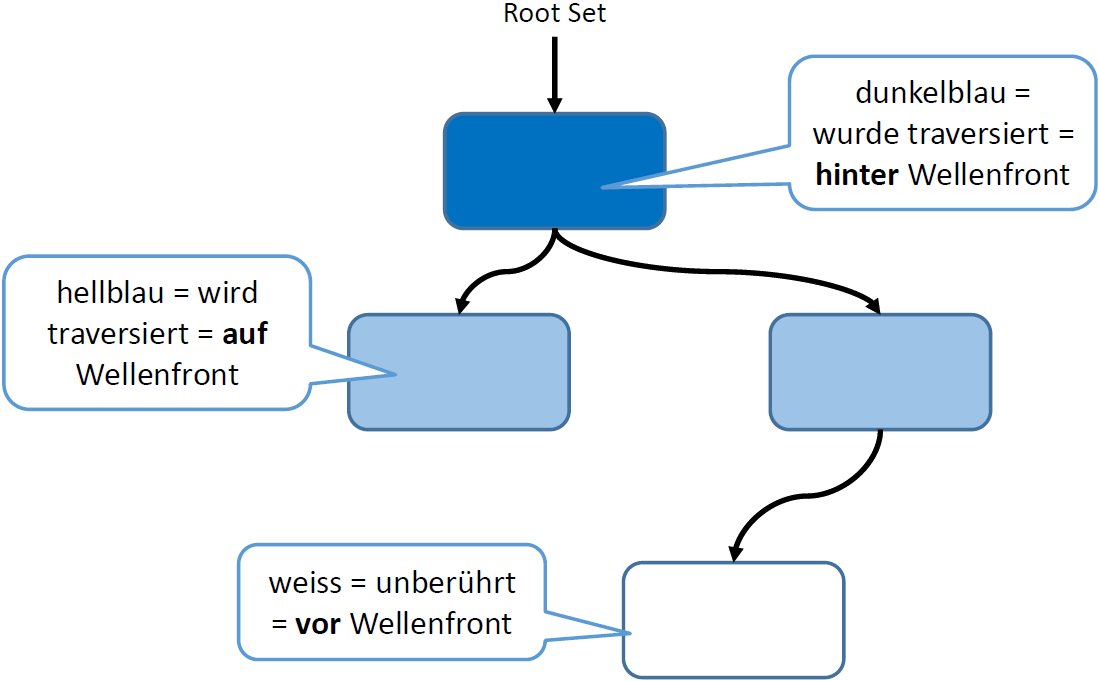
\includegraphics[width=0.6\linewidth]{wellenausbreitungsmodell.png}

\subsection{Isolationsproblem}
\begin{itemize}
    \item Referenzzuweisung durch Mutator während GC
    \item Kritisch: Neue Referenz von dunkelblau zu weiss
    \item \textbf{Heilung:} Quelle oder Ziel hellblau färben (Write Barrier)
\end{itemize}
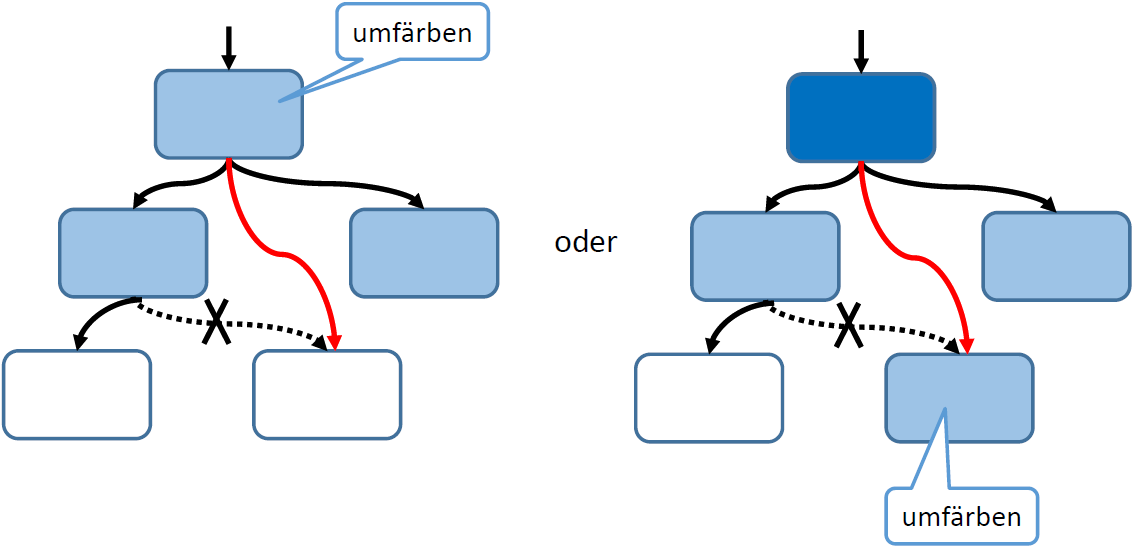
\includegraphics[width=0.6\linewidth]{isolationsproblem.png}
